\begin{figure*}[p]
\centering
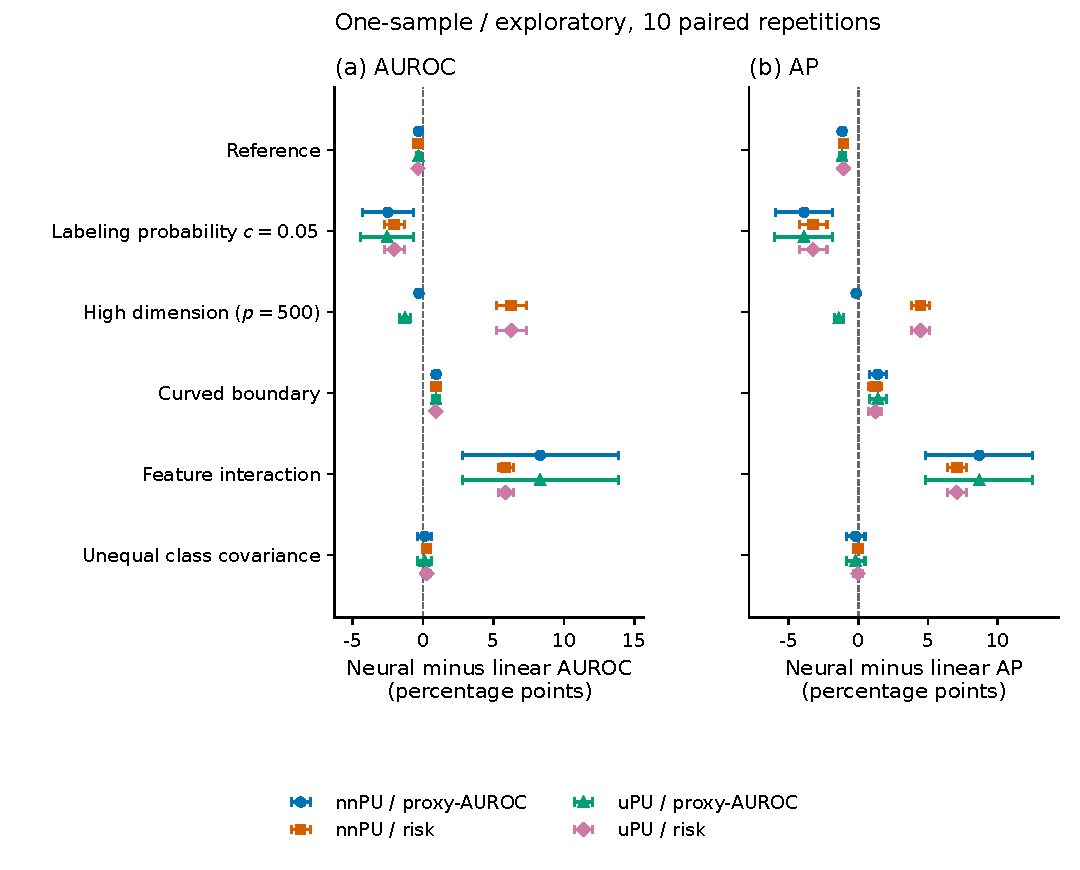
\includegraphics[page=1,width=\textwidth]{revised_figures/fig_s_neural_simulation.pdf}
\caption{Exploratory linear--neural simulation extension: 10 paired repetitions per setting and design. Neural minus matched linear uPU/nnPU is shown separately for risk-based and proxy-AUROC hyperparameter selection. Bars retain the saved pointwise paired t intervals (9 degrees of freedom), not Gaussian large-sample intervals. No BA headline is drawn; these capacity comparisons do not isolate boosting. One-sample / matched linear-neural contrasts. }
\label{fig:s-neural-simulation-1}
\end{figure*}
\begin{figure*}[p]
\centering
\includegraphics[page=2,width=\textwidth]{revised_figures/fig_s_neural_simulation.pdf}
\caption{Exploratory linear--neural simulation extension: 10 paired repetitions per setting and design. Neural minus matched linear uPU/nnPU is shown separately for risk-based and proxy-AUROC hyperparameter selection. Bars retain the saved pointwise paired t intervals (9 degrees of freedom), not Gaussian large-sample intervals. No BA headline is drawn; these capacity comparisons do not isolate boosting. Two-sample / matched linear-neural contrasts. }
\label{fig:s-neural-simulation-2}
\end{figure*}
